% Link to Supplemental Doc:
% https://www.overleaf.com/9488575rxqhnzhzqhgy#/34369899/
% requirements: https://www.nature.com/neuro/pdf/gta.pdf

\documentclass[letterpaper]{article}
%\documentclass[9pt,letterpaper]{article}
\usepackage[top=0.85in,left=1.0in,footskip=0.75in]{geometry}

% Use adjustwidth environment to exceed column width (see example table in text)
\usepackage{changepage}

% Use Unicode characters when possible
\usepackage[utf8x]{inputenc}

% textcomp package and marvosym package for additional characters
\usepackage{textcomp,marvosym}

% fixltx2e package for \textsubscript w
% \usepackage{fixltx2e}

% amsmath and amssymb packages, useful for mathematical formulas and symbols
\usepackage{amsmath,amssymb}

% cite package, to clean up citations in the main text. Do not remove.
\usepackage{cite}
\usepackage{booktabs}

% Use nameref to cite supporting information files (see Supporting Information section for more info)
\usepackage{nameref,hyperref}

% line numbers
\usepackage[right]{lineno}

% ligatures disabled
\usepackage{microtype}
\DisableLigatures[f]{encoding = *, family = * }

% Text layout
\raggedright
\setlength{\parindent}{0.5cm}
\textwidth 6.25in
\textheight 8.75in
\usepackage[aboveskip=1pt,labelfont=bf,labelsep=period,justification=raggedright,singlelinecheck=off]{caption}
\renewcommand{\figurename}{Fig}

\bibliographystyle{plos2015}

% Remove brackets from numbering in List of References
\makeatletter
\renewcommand{\@biblabel}[1]{\quad#1.}
\makeatother

% Leave date blank
\date{}

% Header and Footer with logo
\usepackage{lastpage,fancyhdr,graphicx}
\usepackage{epstopdf}
\pagestyle{myheadings}
\pagestyle{fancy}
\fancyhf{}
\setlength{\headheight}{27.023pt}
\lhead{\sf PNAS Perspectives}
\rfoot{}
\renewcommand{\footrule}{\hrule height 2pt \vspace{2mm}}
\fancyheadoffset[L]{0.0in}
\fancyfootoffset[L]{0.0in}
\lfoot{\sf PNAS Perspectives}


\newcommand{\lorem}{{\bf LOREM}}
\newcommand{\ipsum}{{\bf IPSUM}}

\begin{document}
\vspace*{0.2in}

\begin{flushleft}
{\Large

\textbf\newline{Feasibility theory reconciles alternative approaches to neuromuscular control}
}

% \newline

Brian A. Cohn\textsuperscript{1,\Yinyang},
May Szedl\'{a}k \textsuperscript{2,\Yinyang},
Bernd G{\"a}rtner \textsuperscript{2},
Francisco J. Valero-Cuevas\textsuperscript{3,4*}
\\
\bigskip
\textbf{1} University of Southern California, Department of Computer Science, Los Angeles, CA, USA
\\
\textbf{2} ETH Zurich, Department of Theoretical Computer Science, Zurich, Switzerland
\\
\textbf{3} University of Southern California, Department of Biomedical Engineering, Los Angeles, CA, USA
Current Address: Ronald Tutor Hall, RTH-404
3710 S. McClintock Ave
\\
\textbf{3} University of Southern California, Division of Biokinesiology and Physical Therapy, Los Angeles, CA, USA

Current Address: Ronald Tutor Hall, RTH-404
3710 S. McClintock Ave
Los Angeles, CA 90089-2905, USA % change symbol to "\textcurrency a" if more than one current address note
\\
\Yinyang  B.C. and M.S. contributed equally as first authors.

% Use the asterisk to denote corresponding authorship and provide email address in note below.
* valero@usc.edu

\end{flushleft}
% Please keep the abstract below 150 words for NN
\section*{Abstract}


%%%%%%%%%%%%%%%%%%%%%%%%%%%%%%%%%%%%%%%%%%%%%%%%%%%%%%%%%%%%%%%%%%%%%%%%%%%%%%%%%%%%%%%%%%%%%%%%%%%%%%%%
\pagebreak

%IN NATURE NEURO THE INTRO HEADER IS NOT SHOWN


%%%%%%%%%%%%%%%%%%%%%%%%%%%%%%%%%% Francisco's discussion 5/29
\section*{Discussion}
\subsection*{Summary}

Feasibility theory, as a conceptual and computational approach, is a means to pierce the curse of dimensionality to establish a physics-based ground truth for neuromuscular control. This practical approach can now characterize---in a complete way---the set of all valid ways to activate multiple muscles to produce a given task.
Feasible activation spaces are, in fact, \emph{the} neuromechanical landscapes upon which all neuromuscular learning, control, and performance must occur. Therefore, we provide an integrative and unifying perspective that demonstrates how today's dominant theories of neuromuscular control are alternative approximations to feasible activation spaces from optimization, geometric, and probabilistic perspectives.

\subsection*{The value of a cost function}

Optimization is the oldest computational approach to finding valid muscle activation patterns that produce limb function (e.g.,~\cite{Chao1978Graphical}).
While optimization is a reasonable hypotheses to explore neuromuscular control~\cite{todorov2002optimal}, some criticize it as mathematical abstraction that anthropomorphizes neurons with the ability to choose, evaluate and follow cost functions in high-dimensions~\cite{deRugy2012habitual,loeb2012optimal}.
There is an intimate relationship between optimization and feasible activation spaces~\cite{chvatal1983linear}. Optimization is analogous to finding a best solution in the dark---guided by repeated evaluations of a cost-function. Computing the feasible activation space is then a means to `turn on the lights' to see all possible valid solutions independently of cost~\cite{valero-cuevas2015fundamentals}. Our complete sampling of high-dimensional feasible activation spaces ~\cite{smith1984efficient,lovasz1999hit} allows us to compare and contrast \emph{families} of solutions instead of \emph{individual} optimal solutions for a particular cost function.
Fig.~\ref{fig:figure_4_parcoord} demonstrates a complete description of families of valid coordination patterns and their relationship to alternative costs. Importantly, similar valid muscle activation patterns can have dissimilar costs, and vice versa.

Because these explorations can be done for alternative cost functions, they can provide quantitative overall descriptions of high-dimensional `cost landscapes.'
By not having to insist on (or settle for) individual optimal---or near-optimal---solutions, we now have the same ability the nervous system has to explore, compare and contrast multiple valid ways to coordinate muscles. Importantly, the relationships among valid muscle activation patterns emerge naturally from the physical properties of the limb and definition of the task. This  cost-agnostic approach allows us to re-evaluate our assumptions about what the nervous system cares---and does not care---about. Lastly, this cost-agnostic approach also provides a powerful tool for inverse optimization, i.e., uncovering latent cost functions from data~\cite{tsirakos1997inverse}. Our comparison across cost functions using parallel coordinates is already a form of inverse optimization.

\subsection*{Structure, correlation, and synergies}

The physical properties of the limb and definition of the task also define a low-dimensional structure of the feasible activation space \cite{valero-cuevas2015fundamentals}. Therefore, it is expected that experimental recordings of muscle activations during limb function will exhibit a dimensionality that is smaller than the number of muscles~\cite{kutch2012challenges,alessandro2013musclesynergies}. Thus, applying PCA to the points sampled from the feasible activation space also finds that few PCs can explain the variance in the data.

This application of PCA at increasing task intensities (i.e., as muscle redundancy is lost) allows us to demonstrate---for the first time to our knowledge---several important features and limitations of dimensionality reduction. For example, we see that the aspect ratio (Fig.~\ref{fig:pca_variance_explained}) and orientation (Fig.~\ref{fig:pca_loadings_detail}) of the feasible activation spaces change as their size shrinks (Fig.~\ref{fig:figure_6_histogram_heatmap}).
Thus, such \emph{descriptive} synergies extracted from limited experimental observations likely do not generalize well across task intensities.
It is important to distinguish \emph{descriptive} synergies (the dominant approach in the literature to extract synergies from experimental data using dimensionality reduction techniques such as PCA) from \emph{prescriptive} synergies (those  known to be implemented by the controller)~\cite{valero-cuevas2015fundamentals}.

This also has important consequences to motor control and learning. Producing force vectors at the endpoint of a finger or limb with accurate magnitude and direction are critical for versatile manipulation and locomotion~\cite{cole2006age,valero1998large,donelan2004mechanical}. If a given synergy can produce such accurate force vectors only for a given task intensity (and thus inaccurate ones at other intensities), then the attractiveness of synergies to simplify the neuromuscular control of the limb is reduced.
%That is, if a synergy for low task intensity is used for other intensities, they will produce an inaccurate finger or limb force.
To compensate, the nervous system would need to learn, recall and implement specific synergies for each force level. In prior experimental work, we have shown that the nervous system produces accurate fingertip forces of different magnitudes by, instead, likely scaling a remembered muscle activation pattern to produce forces of different magnitudes, together with a full-dimensional, real-time error correction neural controller~\cite{Valero-Cuevas2000Scaling}. Note that interpreting this experimental result still as a synergy-based approach would defeat the purpose of synergies as a means to simplify the control by reducing its dimensionality.

Our results also show how experiments with realistically moderate numbers of participants and test trials likely do not contain sufficient data to produce robust estimates of descriptive synergies across task intensities. As per the curse of dimensionality, sampling uniformly at random from high-dimensional spaces is exponentially difficult. Thus, even for this anatomically complete 7-muscle finger model, PCA depends strongly on the number of independent observations, such as uncorrelated trials from one subject or different subjects. Figure~\ref{fig:pca_variance_explained} shows that 100 to 1,000 such ideal data points from a simulated `test subject ' are needed to produce accurate estimates of changes in PC1 and PC2 with task intensity (c.f. labels a vs. b vs. c). Future studies should explore how many experimental data points are sufficient from a given subject when recording from only a subset of the many (20+) muscles of human limbs in the presence of experimental noise, inherent stochasticity of EMG, and within- and between-subject variability. Some studies have begun to ask subjects to explore different ways to perform a given task \cite{berger2014effective} (i.e., estimate the structure of the feasible activation space), but in practice such studies cannot likely collect sufficient data uniformly at random to obtain accurate estimates of the descriptive synergies~\cite{kutch2012challenges}. While our results suggest caution when interpreting synergies obtained experimentally, we underscore that dimensionality-reduction is a useful approach to capture global geometric properties of feasible activation spaces.

\subsection*{Toward probabilistic neuromuscular control}

Our results are particularly empowering for the emerging field of probabilistic neuromuscular control~\cite{kording2004bayesian, Kording2014130,berniker2013examination,sanger2011distributed }. Suppose that the nervous system uses some form of probabilistic or Bayesian learning and control strategy. Such approach requires two enabling---and biologically feasible---elements: \emph{trial-and-error iterative exploration}, and \emph{ memory-based exploitation} of the probability density functions used to approximate the feasible activation spaces~\cite{kording2004bayesian}. The parallel coordinate plots and histograms in Fig.~\ref{fig:points_to_parcoords_mapping} and \ref{fig:figure_6_histogram_heatmap} provide, to our knowledge, the first complete~\cite{smith1984efficient,lovasz1999hit} characterization of such multi-dimensional joint probability density functions for a realistic tendon-driven system performing a well-defined task.

These techniques and results now empower the study of fundamental aspects of probabilistic control. For example, an organism can only execute so many trial-and-error iterations during learning, likely too few to completely and exhaustively sample the high-dimensional feasible space of interest. This makes it much more likely that, by virtue of being more easily found, an organism will find and preferentially exploit the strong modes (i.e., narrow and high peaks in Figs.~\ref{fig:figure_4_parcoord}, \ref{fig:parcoord_supplemental}, and \ref{fig:figure_6_histogram_heatmap}) of the multi-dimensional probability density functions than any other region of feasible activation spaces. Thus, first, the maximal ranges of feasible activations described by the bounding box \cite{sohn2013cat_bounding_box,Valero-Cuevas2015high-dimensional} may have little practical bearing on how those tasks are learned and executed. And second, those same strong modes would represent strong attractors to create and reinforce motor habits. Habitual control has been proposed based on experimental and empirical data as an alternative to a strict optimization approach to neuromuscular control~\cite{deRugy2012habitual}. Our work now provides the computational means to link habitual to probabilistic control. This allows us to generate testable hypotheses of how these motor habits are defined by the structure of the feasible activation space, how they are learned by the organism, and how difficult or easy it is to break out of them.

Thus, motor learning likely needs to proceed from adopting easily-found solutions independently of their cost, to using some low dimensional approximation to the gradient of the cost landscape, to then transitioning to less likely but potentially less costly subregions of the solutions space. This integrative perspective leads us to propose a hybrid approach to motor learning and execution where the practical limits on trial-and-error iterations are coupled with the low-dimensional structure of the solution space to enable some form of heuristic local optimization to create sub-optimal motor habits. Importantly, the organism performs strict optimization or synergy control at its peril. Take, for example, the case of a 2-dimensional feasible activation space embedded in 3-D, Fig.~\ref{fig:figure_2_hit_and_run_steps}e. Taking a step from any one valid point to another valid point on the plane runs the risk of `falling off' the solution space and failing at the task---a risk that is exponentially exacerbated in higher-dimensions. Thus, improvements in the neighborhood of a good solution necessarily risk task failure and potential injury. These are all arguments in support of the evolutionary and developmentally useful strategy to use good-enough control based on habit or sensorimotor memory rather than optimization~\cite{deRugy2012habitual, santello2012context}. This may explain why mass practice and coaches are so critical to achieve elite athletic performance~\cite{gladwell2008outliers}.

\subsection*{Clinical implications}
This line of thinking has consequences to neurorehabilitation. Neurological conditions disrupt feasible activation spaces, be it by affecting anatomy of the limb, muscle strength and independence with which muscles can be controlled. Functional recovery following the disruption, if not destruction, of the landscape of valid muscle activation patterns requires re-learning existent, or building new, probability density functions. This occurs just when older adults suffer from reduced perceptuo-motor learning rates \cite{coats201450scliff}.

A probabilistic landscape for neuromuscular function begins to explain why neurorehabilitation in aging adults is so difficult (e.g., ~\cite{hardwick2016motor}) and why motor learning in children takes thousands of repetitions~\cite{adolph2012thousands}---while also generating new rehabilitation strategies, and testable hypotheses around them, that leverage knowledge of the nature and structure of feasible activation spaces.
%%%%%%%%%%%%%%%%%%%%%%%%%%%%%%%%%%
%NATNEURO: "we will continue to ask that authors keep their methods sections to a limit of 2,000 words."
\section*{Online Methods}
The methods to obtain feasible activation spaces for `tendon-driven' limbs are described in detail in the textbook \emph{Fundamentals of Neuromechanics} and references therein~\cite{valero-cuevas2015fundamentals}. This tendon-driven approach explicitly and distinctly avoids the conceptual approach to combine multiple muscle actions into net torques at each joint. Rather, it emphasizes studying the individual actions of all muscles at all levels of analysis, from their neural activation to their contributions to fingertip force. We describe them briefly here.
\label{s:methods}
\subsection*{Theory}
As described in~\cite{valero-cuevas2015fundamentals}, consider a tendon-driven limb, such as a finger, with $n$ independently controllable muscles, where we define the neural command to each muscle as a positive value of activation between 0 (no activation) and 1 (maximal activation).
We can then visualize the set of all feasible neural commands (i.e., all possible muscle activation patterns) as the points contained in a positive n-dimensional cube with sides of length equal to 1. A specific muscle activation pattern is a \emph{point} (i.e., an n-dimensional vector $\textbf{a}$) in this n-dimensional cube~\cite{Chao1978Graphical, spoor1983balancing, Kuo1993Human, Valero-Cuevas1998Large}.
Now consider a specific task, such as producing a vector of static force with the fingertip, as when holding an object. Clearly, not all muscle activation patterns inside the n-dimensional cube can produce that desired static fingertip force vector: The lengths of the bones, the number and type of kinematic degrees of freedom, the anatomical routing of the tendons of each muscle, the posture of the finger, and the relative strengths of the muscles define which subset of points in the n-cube can produce a fingertip force vector of a specific magnitude and direction.
As described in~\cite{Chao1978Graphical, spoor1983balancing, Kuo1993Human, valero-cuevas2015fundamentals} the musculoskeletal anatomy of the limb, the need to control individual tendons, and the physics of a motor task uniquely specify a polytope embedded in $\mathbb{R}^n$ (i.e., the feasible activation space). This polytope contains the family of (potentially infinite) valid muscle activation patterns that can produce this static force production task.
However, these valid muscle coordination patterns are not arbitrarily different because, by construction, the geometric structure of the polytope that contains them defines strict spatial correlations among them~\cite{kutch2012challenges}.

\paragraph*{System of linear equations to simulate static force production by a tendon-driven system}

Consider producing a vector of static force with the endpoint of the limb in a given posture. The constraints that define that task (i.e., the direction and magnitude of the force vector at the endpoint) are linear equations~\cite{valero-cuevas2015fundamentals} that come from the mapping between neural activation of individual muscles to static endpoint forces and torques the limb can produce. This mapping is linearly modeled by the equation
\begin{align}
\label{eq:constraints}
		 \begin{pmatrix}
f_{x}\\
f_{y}\\
f_{z}\\
\tau_{x}\\
\tau_{y}\\
\tau_{z}
\end{pmatrix}=\textbf{w} = H\textbf{a} = H\begin{pmatrix}
a_{1}\\
a_{2}\\
a_{3}\\
...\\
a_{n}
\end{pmatrix}
, \textbf{a} \in [0,1]^n
\end{align}
where $H$ is the matrix of linear constraints defined by the musculoskeletal anatomy of the limb~\cite{Valero-Cuevas2015high-dimensional}, \textbf{a} is the input vector of $n$ muscle activations, $\textbf{f} \in \mathbb{R}^m$ is the m-dimensional limb output `wrench' (i.e., the forces and torques the finger can produce at the endpoint).

The output wrench, $m$, is at most 6-dimensional (i.e., 3 forces and 3 torques) depending on the number of kinematic degrees of freedom of the limb, and usually $m < n$ because limbs have more muscles than kinematic degrees of freedom~\cite{valero-cuevas2015fundamentals}. Muscles can only pull, so elements of \textbf{a} cannot be negative, and are capped at 1 (i.e., 100\% of maximal muscle activation).

What are the muscle coordination patterns that produce a given task? As explained in~\cite{valero-cuevas2015fundamentals}, the task of producing a static fingertip force vector is defined by specifying the desired values for the elements of the endpoint forces and torques of $\textbf{w}$. Each such constraint equation defines a hyperplane of dimension $n-1$, and their combination defines the task completely. The \emph{feasible activation space} of the task, if it is well posed~\cite{chvatal1983linear}, is defined by the points $\textbf{a}$ that lie within the $n$-cube and at the intersection of all constraint hyperplanes.

Geometrically speaking, the feasible activation space is a $(n-m)$-dimensional convex polytope $P$ embedded in $\mathbb{R}^n$ that contains all n-dimensional muscle coordination patterns (i.e., points $\textbf{a}$) that satisfy all constraints, and therefore can produce the task. Increasing task specificity by adding more constraints naturally decreases the dimensionality and changes the size and shape of the feasible activation space~\cite{Kuo1993Human,sohn2013cat_bounding_box,inouye2016muscle}.


\paragraph*{The Hit-and-Run algorithm uniformly samples from feasible activation spaces}
\label{ss:hitrun}

The goal is to characterize the qualities that define all valid muscle activation patterns (i.e., n-dimensional vectors $\textbf{a}$), that are points that make up $P$. This is equivalent to characterizing the structure of the convex polytope $P$. But calculating the geometric properties of convex polytopes in high dimensions is computationally challenging. Taking the generalized concept of an $n$-dimensional volume as an example of a geometric property of interest, the exact volume computations for n-dimensional polytopes is known to be tractable only in a polynomial amount of time (i.e., $\#P$-hard)~\cite{Dyer}.
Currently available volume algorithms can only handle polytopes embedded in small dimensions like 10 or slightly more~\cite{Bueler2}. Studying vertebrate limbs in general, however, can require including several dozen muscles, such as our studies of a 17-muscle human arm and a 31-muscle cat hindlimb model~\cite{Valero-Cuevas2015high-dimensional}; and other limb models have over 40 muscles such as~\cite{arnold2010model, kutch2012challenges, hamner2010muscle, de2014human}.

Similar difficulties arise when computing other geometric properties such as the shape and aspect ratio of $P$ in high dimensions. We and others have described polytopes $P$ by their bounding box (i..e, the range of values in every dimension)~\cite{sohn2013cat_bounding_box,kutch2011muscle}, but that singularly overestimates the shape and volume of the feasible activation space as discussed in~\cite{Valero-Cuevas2015high-dimensional}.
Take Fig.~\ref{fig:figure_2_hit_and_run_steps}e as an example, where the bounding box of the 2-dimensional polygon has a volume---even though a plane has zero volume---, and can be almost as large as the positive unit cube itself. Similar problems arise in the interpretation of the inscribed and circumscribed ball~\cite{inouye2014optimizing}.

\begin{figure}[htbp]
\centering
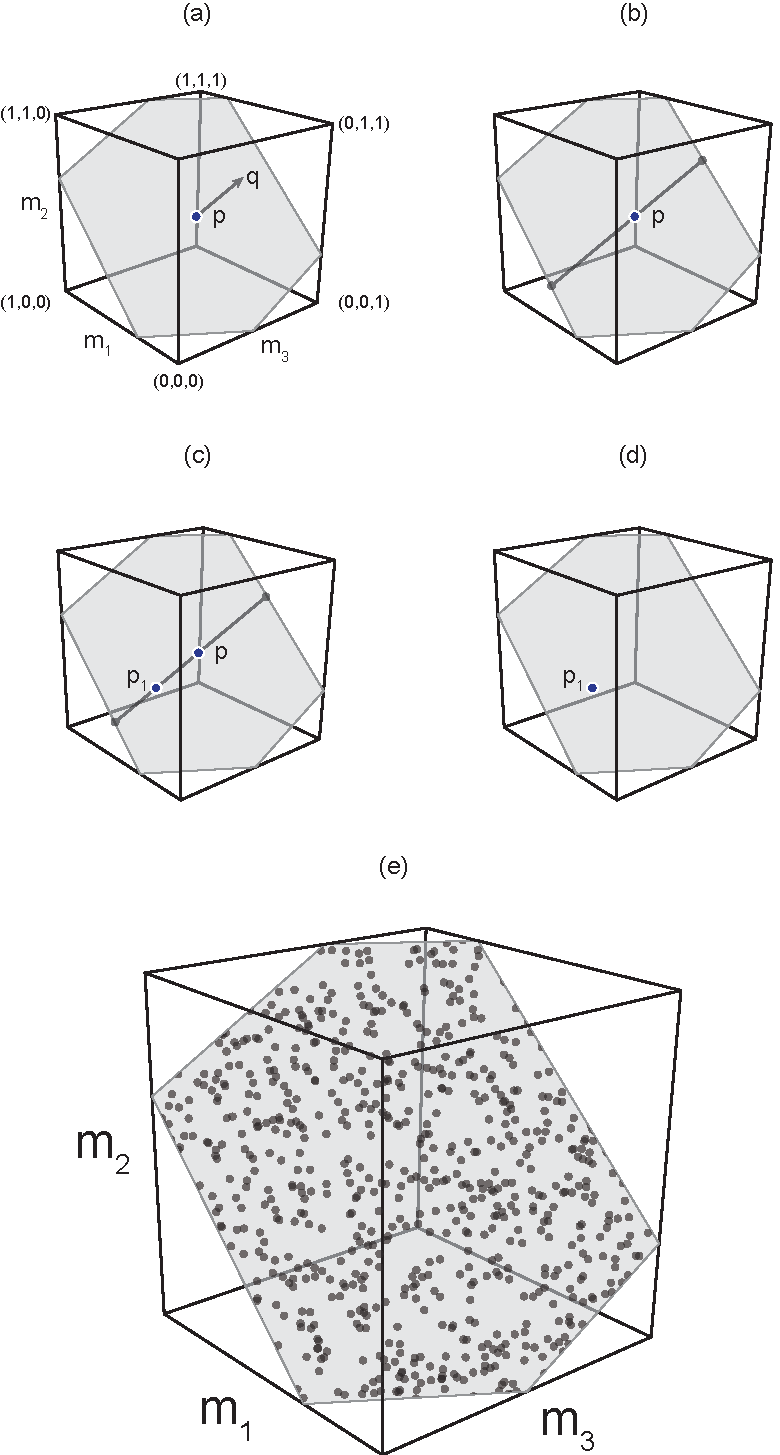
\includegraphics[width=0.5\textwidth]{numbered_figures/figure_2_hit_and_run_ALL_steps.pdf}
\caption{\textbf{Characterizing the high-dimensional structure of a feasible activation set via the Hit-and-Run algorithm~\cite{lovasz1999hit}.}  For a large class of biomechanical tasks, the feasible activation set is a convex polytope. Here we show a 3-muscle system as a schematic example upon which Hit-and-Run can be applied. We select a valid direction at random (a), and project a line to both boundaries (b). After selecting a point at random from the resulting line (c), we get a new valid point $p_1$ (d). Repeating steps a-d many (e.g., 100,000) times, and down-sampling those points, produces a statistically complete representation of the polytope (e)---and of the high-dimensional structure of the feasible activation set.}
\label{fig:figure_2_hit_and_run_steps}
\end{figure}


We propose a complete probabilistic method to describe the structure of feasible activation spaces $P$. This includes the the descriptive statistics, histograms, and point densities of the set of valid muscle activation patterns $\textbf{a}$ uniformly sampled from the polytope. To do so, we use the Hit-and-Run method. Experimentally, it is known to converge to a uniform sampling across any convex body, up to about 40 dimensions~\cite{smith1984efficient}. The Hit-and-Run method is a generalization of a discrete Markov chain---where the goal is to identify multiple points from the feasible activation polytope $P$ uniformly-at-random.

The Hit-and-Run algorithm is defined as follows (it works analogously for any convex body even if not a polytope)\cite{lovasz1999hit}:
\begin{enumerate}
\item Find a point $\textbf{p}$ in $P$ to use as a starting point by using the linear programming method documented in the Supplementary Note.
\item Generate a line in a random direction $q$ (uniformly-at-random\ over all directions) from $\textbf{p}$ in $P$ (Fig.~\ref{fig:figure_2_hit_and_run_steps}a).
\item Find the two intersection points of the line given by the random direction $q$ with the boundary of the polytope (Fig.~\ref{fig:figure_2_hit_and_run_steps}b).
\item Choose a new point uniformly-at-random on the line segment between the intersection points (Fig.~\ref{fig:figure_2_hit_and_run_steps}c).
\item Repeat the above steps from $2.$ onwards using the new point as the starting point, and generate a new random direction.
Continue this process for $s$ iterations, where $s$ is the mixing number. The mixing number is the number of iterations that are expected to result in a point sampled uniformly at random from the space, with respect to the starting point (and any other point in $P$. Saving just the $s^{th}$ point for many repetitions will result in many uniform-at-random points collected across the feasible activation space (Fig.~\ref{fig:figure_2_hit_and_run_steps}).
\end{enumerate}

We describe the mathematical basis and details to replicate our implementation in the Supplementary Note, including our application of slack variables to select a valid starting point within the feasible activation space.

\subsection*{Example of a tendon-driven system}
\paragraph*{Realistic 3-D model of a 7-muscle human index finger}
\label{ss:finger}
We applied this methodology to our published model of an index finger for static fingertip force production.
The model is described in detail elsewhere~\cite{valero-cuevas2009computational}.
Briefly, the input to the model is a 7-D muscle activation pattern $\textbf{a}$, and the output is a 4-D wrench (i.e., static forces and torque) at the fingertip $\textbf{w}$

\begin{eqnarray}
\textbf{w} = H \textbf{a} \\
H=J^{-T}RF_o \\
H \in \mathbb{R}^{4 \times 7}
\end{eqnarray}

where

\begin{equation}
\label{eq:a}
\textbf{a}=
\begin{pmatrix}
a_{FDP}\\
a_{FDS}\\
a_{EIP}\\
a_{EDC}\\
a_{LUM}\\
a_{DI}\\
a_{PI}
\end{pmatrix}
\end{equation}

In Cartesian coordinates, the output wrench is

\begin{equation}
\label{eq:wc}
\textbf{w}=
\begin{pmatrix}
f_{x}\\
f_{y}\\
f_{z}\\
\tau_{x}
\end{pmatrix}
\end{equation}

which corresponds to these anatomical directions shown in Fig.~\ref{fig:overview}e.
\begin{equation}
\label{eq:wa}
\textbf{w}=
\begin{pmatrix}
f_{radial}\\
f_{distal}\\
f_{palmar}\\
\tau_{radial}
\end{pmatrix}
\end{equation}

The biomechanical model $H$ includes three serial links articulated by four kinematic degrees of freedom (ad-abduction, flexion-extension at the metacarpophalangeal joint, and flexion-extension at the proximal and distal interphalangeal joints). The action of each of the seven muscles (FDP: \emph{flexor digitorum profundus}, FDS: \emph{flexor digitorum superficialis}, EIP: \emph{extensor indicis proprius}, EDC: \emph{extensor digitorum communis}, LUM: \emph{lumbrical}, DI: \emph{dorsal interosseous}, and PI: \emph{palmar interosseous}) on each joint to produce torque is given by the moment arm matrix $R \in \mathbb{R}^{4 \times 7}$. Lastly, $J \in \mathbb{R}^{4 \times 4}$ and $F_0 \in \mathbb{R}^{7 \times 7}$ are the Jacobian of the fingertip with 4 kinematic degrees of freedom, and the diagonal matrix containing the maximal strengths of the seven muscles, respectively~\cite{valero-cuevas2015fundamentals,Valero-Cuevas2000Scaling}. The finger posture was defined to be $0^\circ$ ad-abduction and $45^\circ$ flexion at the metacarpophalangeal joint, and $45^\circ$ and $10^\circ$ flexion, respectively, at the proximal and distal interphalangeal joints.

\paragraph*{Feasible activation space for a static fingertip force task}

Our goal is to find the family of all feasible muscle activation patterns that can produce a given task. In particular, the task we explored is producing various magnitudes of a submaximal static force in the distal direction $f_{distal}$ --- in the absence of any $\tau_{radial}$, shown in Fig.~\ref{fig:overview}f. Therefore the feasible activation space is a polytope $P$ in 7-dimensional activation space that meets the following \emph{four} linear constraints in $\textbf{a}$~\cite{Valero-Cuevas1998Large,valero-cuevas2015fundamentals,Valero-Cuevas2000Scaling}

\begin{eqnarray}
f_{radial} = 0 \\
f_{distal} = \emph{desired magnitude as \% of maximal} \\
f_{palmar} = 0 \\
\tau_{palmar} = 0
\end{eqnarray}

These four constraints on the static output of the finger yield a 3-dimensional (i.e., $7-4=3$) polytope $P$ embedded in 7-dimensional activation space.
For details on how to create such models, apply task constraints and find such polytopes via vertex enumeration methods, see~\cite{valero-cuevas2015fundamentals}.

Thus all valid output wrenches will have the form

\begin{equation}
\label{eq:wrench}
\textbf{w}=
\begin{pmatrix}
0\\
\text{Desired distal task intensity in N} \\
0\\
0
\end{pmatrix}
\end{equation}

For the index finger model used in this paper, the published maximal feasible force in the distal direction is 28.81 Newtons. We defined the normalized desired distal task intensity as a value ranging between $0$ and $1$, i.e., each submaximal force can be produced by any of the points contained in its corresponding feasible activation space. For the production of a maximal force with $\alpha=1$ the feasible activation space shrinks to a single point~\cite{spoor1983balancing,Chao1978Graphical,chvatal1983linear,Valero-Cuevas2000Scaling}.

\subsection*{Analysis of feasible activation spaces}
\paragraph*{Parallel coordinates visualization shows the location of all points across all dimensions}

Parallel coordinates are a common graphical approach to visualize interactions among high-dimensional data, which has been used in biomechanical studies~\cite{bachynskyi2013biomechanical, krekel2010visual}.
To demonstrate this visualization method, consider the results of the simple 3-dimensional example shown in Fig.~\ref{fig:figure_2_hit_and_run_steps}e. We begin by drawing $n$ parallel vertical lines for each of the dimensions $n$ (i.e., 3 muscles).
With the axis limits of each line set between 0 and 1, each point (Fig.~\ref{fig:points_to_parcoords_mapping}a) is then represented by connecting their coordinates by $n-1$ lines as shown in Fig.~\ref{fig:points_to_parcoords_mapping}b.

\paragraph*{Neural and metabolic cost functions}

As mentioned in the Introduction, the field of neuromuscular control has a long historical tradition of using optimization to find muscle activation patterns that minimize effort, which requires the (often contentious) definition of cost functions~\cite{spoor1983balancing,Chao1978Graphical,Prilutsky2000Muscle,crowninshield1981physiologically}. Therefore, we used four representative cost functions to calculate the relative fitness of each of the muscle activation patterns sampled---in effect also calculating the fitness landscape across all possible solutions. The cost functions are defined at the level of neural effort ($L_1$, and $L_2$ norms); and at the level of metabolic cost, thought to be approximated by neural drive weighted by the strength of each muscle ($L_1^w$ and $L_2^w$ norms)~\cite{Prilutsky2000Muscle,crowninshield1981physiologically}.

To visualize the costs associated with each valid muscle coordination pattern, we simply added four vertical lines at the far right of the parallel coordinates plot, one for each cost function, Fig.~\ref{fig:points_to_parcoords_mapping}c. The variables $a_i$ and $F_{0i}$ represent the activation of the $i^{th}$ muscle in a given muscle activation pattern, and the maximal strength of each muscle~\cite{Prilutsky2000Muscle,crowninshield1981physiologically}. Maximal muscle strengths are approximated by the multiplying each muscle's physiological cross-sectional area, in $cm^2$, by the maximal active muscle stress of mammalian muscle, $35~N/{cm^2}$~\cite{Zajac1993Muscle}. These four cost functions are but four examples as the literature contains many others as any investigator is in fact free to chose any cost function deemed relevant to their study.


\paragraph*{Histograms of the activation level of each muscle across all valid solutions}

Muscle-by-muscle histograms are another straightforward way to visualize the many points sampled from the convex polytope. Histograms are particularly helpful because they are approximations to probability density functions.
They visualize the relative number of solutions (i.e., density of solutions) that required a particular level of activation from a particular muscle within its range of $[0,1]$.
In addition, the upper and lower bounds of the histograms show, in fact, the size of the side of the bounding box of the polytope in every dimension (i.e., for independently controlled muscle).

\paragraph*{Dimensionality reduction}

Investigators have repeatedly reported that electromyographical signals (i.e, experimental estimates of muscle activation patterns) tend to exhibit strong correlations with one another.
In these experimental descriptions of dimensionality reduction of neuromuscular control, only few independent functions---sometimes called synergies---suffice to explain the majority of the variability in the observed muscle activation patterns~\cite{kutch2012challenges,steele2013number,bizzi2013neural,dingwell2010walkingvariability,steele2015consequences,alessandro2013musclesynergies,krishnamoorthy2003muscle}.
Principal components analysis (PCA) is a widely used technique to extract these few independent basis functions (correlation vectors called principal components, PCs) from high-dimensional data~\cite{Clewley2008Estimating}.
In this case, PCs are often called the experimental representations of synergies of neural origin~\cite{kutch2012challenges}.

Therefore, we also applied PCA to points (i.e., muscle coordination patterns) sampled from the feasible activation space at each force level.
This provides the PCs that describe the correlations among valid muscle activation patterns for a given task.
For example, the feasible activation space $P$ in Fig.~\ref{fig:figure_2_hit_and_run_steps}e is a 2-dimensional polygon embedded in 3-dimensional activation space. Thus, applying PCA to points sampled from the polygon will extract 2 synergies (i.e., 3-dimensional correlation vectors PC1 and PC2) that wholly explain the feasible activation space. By extension, in the case of fingertip force production in Fig.~\ref{fig:overview}, the feasible activation space is a 3-dimensional polytope embedded of the 7-dimensional activation space. And PCA should extract, by construction, as many synergies as there are dimensions in the feasible activation space. For static force production with the index fingertip (i.e., 7 muscles and 4 constraints), we know that 3 principal components should describe 100\% of the variance in points sampled from the feasible activation space (i.e., 7-dimensional correlation vectors PC1, PC2, and PC3).

Applying PCA to our data allows us to test whether and how its results change when applied to feasible activation spaces for different magnitudes of fingertip force. We applied PCA to feasible activation spaces for fingertip task intensities ranging from 0 to 90\% of maximal.
We compare both the variance explained by each PC and their vector direction (i..e, the `loadings' or correlations among muscle~\cite{valero2016robot}) as the force level increases.
Lastly, we tested whether our PCA results are sensitive to the number of points sampled from each feasible activation space. This is important because experimental studies test 10 or so subjects in practice, which may be too few when sampling from high-dimensional spaces.


\section*{Supplementary Note: Algorithmic Implementaion of Hit-and-Run}
The polytope $P$ is defined by the mechanics of the limb and the constraints of the task as
\[\textbf{f} = A\textbf{a}, \textbf{a} \in [0,1]^n,\]
and to find a starting point $\textbf{p}$ we need only to find one feasible activation vector in the space.
For the Hit-and-Run algorithm to mix faster we do not want the starting point to be close to a vertex of $P$ ~\cite{Lovasz}. Intuitively, this is because we do not want to get stuck in a corner.
We use the following standard trick with slack variables $\epsilon_i$, which in practice often provides a good starting point for sampling algorithms. In essence, we use the slack variables to find a point far away from the boundaries of the $n$-cube.

\begin{equation}\label{eq:LP_r}
\begin{array}{lrcl}
\mbox{maximize} & \sum_{i=1}^n \epsilon_i \\
\mbox{subject to} & \textbf{f} &=& A\textbf{a}\\
 & a_i &\in& [\epsilon_i, 1- \epsilon_i], \hspace{5mm} \forall i \in \{1,\dots,n\} \\
 & \epsilon_i &\geq& 0, \hspace{5mm} \forall i \in \{1,\dots,n\}.
\end{array}
\end{equation}
Thus running a linear program with these reduced ranges of the variables will produce a starting point that is far from the boundaries of $P$, and is not stuck in a corner.



The rest of the implementation of the Hit-and-Run algorithm is straightforward except for the choice of the random direction $q$. How do we sample u.a.r.\ (uniformly-at-random) from all directions in $P$?
Recall that all points in $P$ are by definition valid solutions to a given task.

The direction of $q$ must be in the null space of the task, which is defined as $V = \{ y \in R^n \mid Ay = 0\}$. Hence we need to choose  directions uniformly at random across the vector space $V$.

As shown by Marsaglia this can be done as follows~\cite{Marsaglia}.
\begin{enumerate}
\item
Find an orthonormal basis $b_1, \dots, b_r \in \mathbb{R}^{n}$ of \{$\textbf{q} \in \mathbb{R}^n | A\textbf{q} = 0$\}.
\item
Choose $(\lambda_1, \dots, \lambda_r) \in \mathcal{N}(0,1)^r$ (from the zero-mean unit-variance Gaussian distribution).
\item
$\sum_{i=1}^r \lambda_i b_i$ is a u.a.r.\ direction.
\end{enumerate}

A basis of a vector space $V$ is a minimal set of vectors that generate $V$, and it is orthonormal if the vectors are pairwise orthogonal (perpendicular) and have unit length. Using basic linear algebra one can find a basis for $\{q \in \mathbb{R}^n | A\textbf{q} = 0\}$ and orthogonalize with the well known Gram-Schmidt method. Note that in order to get the desired uniform and random sample the basis needs to be orthonormal. The limb model is defined such that the rows of $A$ are linearly independent and hence $r=n-m$.

\subsection*{Mixing Time}
\label{sec_lengthrun}
While we have rigorous experimental evidence that supports using Hit-and-Run in this setting, we do not have theoretical proof that guarantees our sampling will mix to the uniform distribution. Hit-and-Run is theoretically guaranteed to mix in time $\mathcal{O}(n^3)$ if the polytope is not too "flat", meaning that the ratio between the inscribed circle and enclosing circle is not too small. Such degenerate examples are usually artificially created and we henceforth assume that this does not happen in our system of muscles.
From a given starting point, how many iterations of the Hit-and-Run method are necessary to reach a u.a.r.\ point?
For convex polytopes in $n$ dimensions up to $40$, experimental results suggest that $\mathcal{O}(n)$ steps of the Hit-and-Run algorithm are sufficient.
In particular, the paper~\cite{emiris2013efficient} by Emiris and Fisikopoulos suggests that selecting every $10(n + 1)$ points is sufficient to get a uniform distribution~\cite{emiris2013efficient}, while in Ge et al.'s paper every single point of the Hit-and-Run algorithm is used in the sample~\cite{Ge}. It's worth noting that these results are experimental, not theoretical.


The Hit-and-Run algorithm was specifically developed to address $\#P$-hard problems such as approximating the volume of high-dimensional polytopes\cite{Dyer}. The Hit-and-Run algorithms can converge to the uniform sampling across any convex body~\cite{smith1984efficient} after $\mathcal{O}^*(n^2R^2/r^2)$ steps ($r$ and $R$ are the radii of the inscribed and circumscribed ball of the polytope as mentioned in the Introduction)~\cite{Dyer, Lovasz}. Experimental results suggest that a number of points linear with respect to $N$ suffices for convex polytopes embedded in dimensions up to 40. Emiris and Fisikopoulos~\cite{emiris2013efficient} suggest that $(10 + \frac{10}{N})~N$ iterations suffice to uniformly sample a convex polytope.

\subsection*{Data and code availability}
All analyses are replicable and extensible with Open Source libraries. We developed and tested our code in Ubuntu 14.04, Windows 8.1, and OSX Yosemite 10.12.1; implemented Hit-and-Run with Scala 2.11.6, and developed visualizations with R 3.3.0.
All figure source data are available within the repository https://github.com/briancohn/space.

\section*{Acknowledgments}
Research reported in this publication was supported by the National Institute of Arthritis and Musculoskeletal and Skin Diseases of the National Institutes of Health (NIH) under Awards Number R01 AR-050520 and R01 AR-052345 to FVC, and the Swiss National Science Foundation (SNF Project 200021\_150055 / 1) to BG, KF and FVC. The content is solely the responsibility of the authors and does not necessarily represent the official views of the SNSF or the NIH. We thank Komei Fukuda for his integral support in designing this research collaboration. We thank J Pugliesi, T Kim, C Lim, A Baugus, P Vachhani, and A Boling for extending the scientific rigor of this work through reviews, documentation, and code.

\section*{Author contributions and Correspondence}
M.S. derived the mathematics of our Hit-and-Run implementations, B.C. implemented those algorithms and designed the simulations. F.V.C supported the neurobiological interpretations, while B.G. supported work with computational geometry. F.V.C. can be contacted via valero@usc.edu.

\section*{Competing Financial Interests}
We do not have any competing interest to declare.

% \nolinenumbers

\bibliography{plos_cohn_bibliography.bib}
% \bibliographystyle{plain}

\end{document}
